\documentclass[10pt,final,leqno]{beamer}

%\usetheme{CambridgeUS}
\usetheme[style=ntnu,language=en]{ntnu2015}
%\usecolortheme{orchid}

\usepackage[utf8]{inputenc}
\usepackage[T1]{fontenc}

% Paths
\newcommand{\figs}{../figs}
\newcommand{\data}{../data}
\newcommand{\code}{../code}

% URL styles
\usepackage{url}
\urlstyle{sf}

% Units
\usepackage[detect-weight=true, binary-units=true]{siunitx}
\DeclareSIUnit\flop{FLOPS}

% Math
\usepackage{amsmath}
\usepackage{amssymb}
\usepackage{bm}
\usepackage{nicefrac}
\newcommand{\dif}[1]{{\;\text{d}#1}}

% Graphics
\usepackage{graphicx}
\usepackage{caption}
%\usepackage{subcaption}
\graphicspath{{../figs/}}

% Tikz
\usepackage{tikz}
\usetikzlibrary{positioning,shapes,arrows,calc,intersections}
\usepackage{pgfplots}
\usepgfplotslibrary{dateplot}
\pgfplotsset{compat=1.14} 

% Colors
\definecolor{darkblue}{HTML}{00688B}
\definecolor{darkgreen}{HTML}{6E8B3D}
\definecolor{cadet}{HTML}{DAE1FF}
\definecolor{salmon}{HTML}{FFB08A}

\usepackage{algorithm}

% Listings
\usepackage{textcomp}
\usepackage{listings}
\lstset{
  keywordstyle=\bfseries\color{orange},
  stringstyle=\color{darkblue!80},
  commentstyle=\color{darkblue!80},
  showstringspaces=false,
  basicstyle=\ttfamily,
  upquote=true,
}
\lstdefinestyle{fortran}{
  language=Fortran,
  morekeywords={for},
  deletekeywords={status},
}
\lstdefinestyle{c}{
  language=C,
  morekeywords={include},
}
\lstdefinestyle{glsl}{
  language=C,
  morekeywords={attribute, vec2, vec3, vec4, varying, uniform, mat2, mat3, mat4},
}
\lstdefinestyle{cuda}{
  language=C,
  morekeywords={__global__, __device__, __host__, __shared__},
}
\lstdefinestyle{shell}{
  language=bash,
  morekeywords={mkdir, ssh, cmake},
}

% Double hlines
\usepackage{hhline}

% Misc
\usepackage{nth}

\subtitle{TMA4280---Introduction to Supercomputing}

\graphicspath {{../figs/}}

\AtBeginSection[]
{
 \begin{frame}<beamer>
 \frametitle{Outline}
 \tableofcontents[currentsection]
 \end{frame}
}

\begin{document}


\title{Course description}
\institute{NTNU, IMF}
\date{January 10. 2018}
\author{Aurélien Larcher}
\maketitle

\begin{frame}
  \frametitle{Schedule}

14 sessions: Week 2--12 then 14-16
\medskip

\begin{center}
\begin{tabular}{|l|l|l|}
\hline
Lectures   & Friday 12--15    & B1          \\
Exercises  & Wednesday 17--19 & Banachrommet \\
\hline
\end{tabular}
\end{center}

Notes:
\begin{itemize}
\item Except the Curriculum presentation on Week 2, \textbf{all} Labs will be located at the computer room Banachrommet.
\item Weeks 3 and 4 will serve as introduction and get everyone started with programming and numerics.
\item Office hours are offered on:
\begin{enumerate}
\item Thursday 17-19
\item Friday 15-17
\end{enumerate}
\item Please book the office hours latest on Tuesday.
\end{itemize}

\end{frame}

\begin{frame}
  \frametitle{Evaluation}

\begin{tabular}{|l|l|l|l|}
\hline
$40\%$ & Projects    & 1. Basic programming          ($10\%$) & 2018-03-07 \\
       &             & 2. MPI/OpenMP                 ($30\%$) & 2018-04-20 \\                        
$60\%$ & Examination & Three problems & 2018-05-16 \\
\hline 
\end{tabular}

\medskip
Projects:
\begin{enumerate}
\item Delivery involves written report \textbf{and} source code.
\item Final handout consists of a commented project demo (approx. 5 min).
\item Other Labs are optional but obviously recommended.
\end{enumerate}

\medskip
Examination:
\begin{enumerate}
\item Small exercises during the Labs will cover most requirements.
\item Previous examination question studied during the lectures.
\item Repetition session scheduled at the end of the curriculum.
\end{enumerate}

\end{frame}

\begin{frame}
  \frametitle{Course plan}

Two main parts:
\begin{enumerate}
\item Computer architectures and programming models.
\item Application to numerical algorithms.
\end{enumerate}

\medskip
\begin{itemize}
\item The first part is usually easily understood by Computer Science students, but should not scare others away: the important is to understand the underling concepts. This is not a CS course.
\item The second part is usually the other way around, but the mathematical requirements are kept at the application level.
\end{itemize}

\end{frame}


\begin{frame}
  \frametitle{Course plan: Part 1}

Computer architectures and programming models:
\begin{enumerate}
\item W2: Introduction to Supercomputing:
\begin{itemize}
\item Why is Supercomputing needed?
\item What is the evolution of parallel computers and algorithms?
\item What is the future of Supercomputing?
\end{itemize}
\smallskip
\item W3: Computer architectures I : Single-Processor
\begin{itemize}
\item What is the definition of a processing unit?
\item What are the different ways to take advantage of parallelism?
\end{itemize}
\smallskip
\item W4: Computer architectures II: Multi-Processor
\begin{itemize}
\item What are the different possible extensions to multiprocessing?
\item What are the advantages and limits?
\item How to analyse the performance of an algorithm or a system?
\end{itemize}
\smallskip
\item W5-6: Distributed memory model: MPI (Message Passing)
\item W7-8: Shared memory model: OpenMP (Multithreading)
\end{enumerate}

\end{frame}


\begin{frame}
  \frametitle{Supercomputing: history and trends}
  \begin{center}
    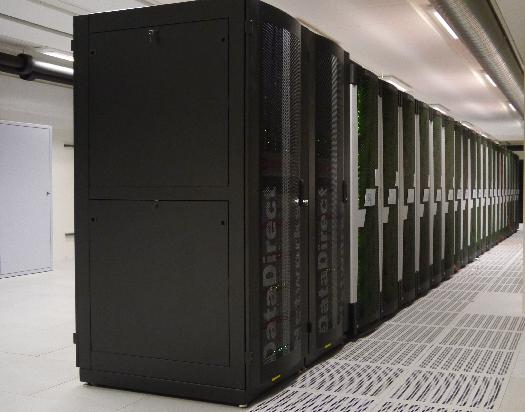
\includegraphics[height=0.6\textheight]{\figs/tma4280/vilje}
  \end{center}

Past evolution, relation to numerical algorithms, and perspectives.
\end{frame}


\begin{frame}
  \frametitle{An introduction to UNIX and C/C++ Programming}
  \begin{center}
    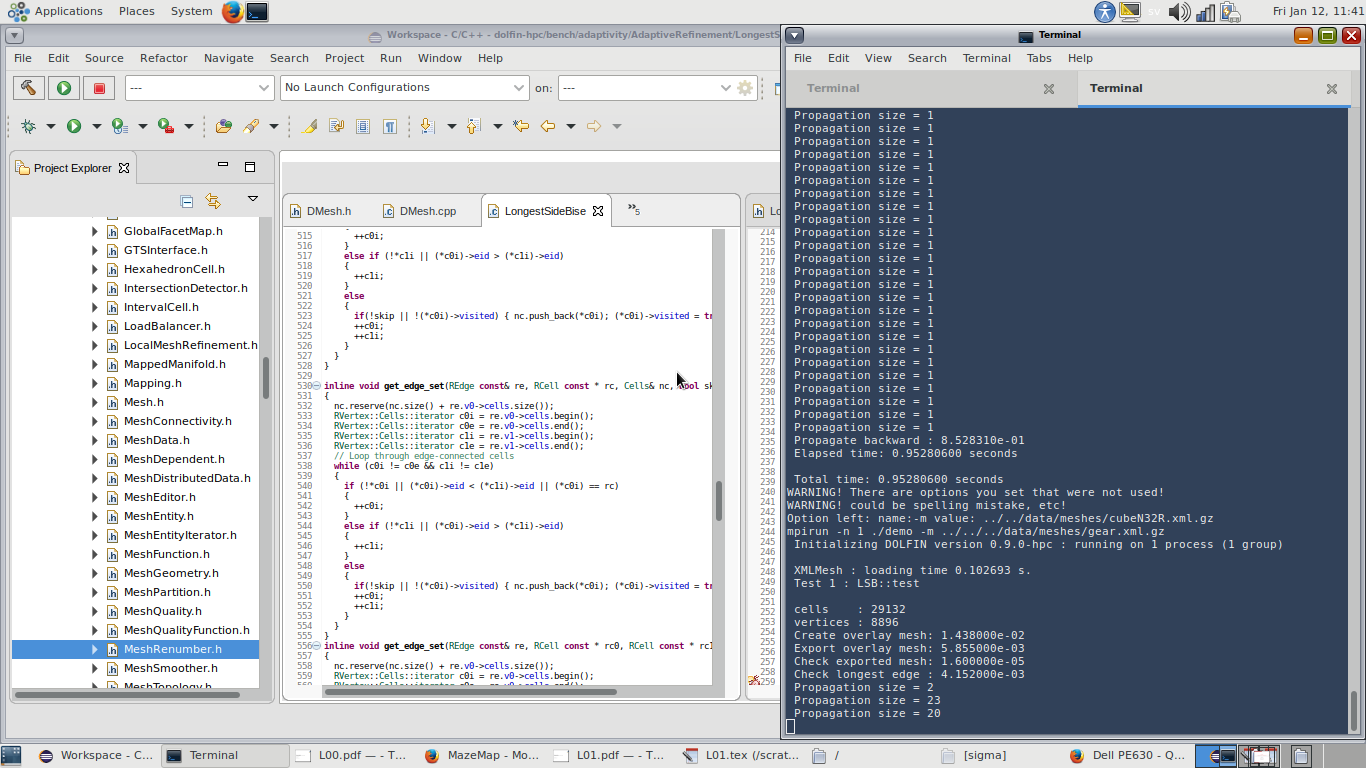
\includegraphics[width=10cm]{\figs/tma4280/eclipse}
  \end{center}

Recommended practice to prepare for the projects.
\end{frame}

\begin{frame}
  \frametitle{Computing architectures}
  \begin{center}
    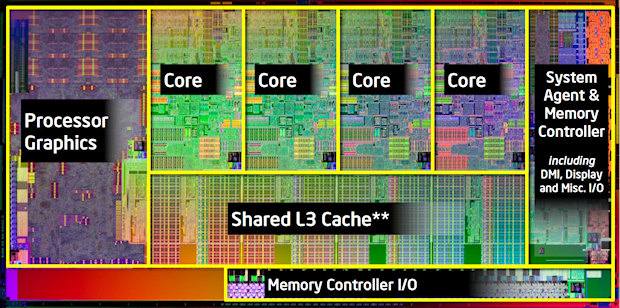
\includegraphics[height=0.6\textheight]{\figs/tma4280/sandy}
  \end{center}

Introduction to floating-point computations and description of different levels of parallelism available on hardware.
\end{frame}

\begin{frame}[fragile]
  \frametitle{Distributed memory programming with MPI}
  \begin{center}
    \texttt{node 0: Hello, world} \\
    \texttt{node 1: Hello, world} \\
    \texttt{node 3: Hello, world} \\
    \texttt{node 2: Hello, world}
  \end{center}
  \begin{center}
    
\includegraphics[width=3cm]{\figs/tma4280/open-mpi-logo}
  \end{center}

\vspace{4em}
Development of parallel algorithms on distributed memory systems: message passing paradigm, performance analysis.
\end{frame}

\begin{frame}
  \frametitle{Shared memory programming with OpenMP}

\vspace{4em}
  \begin{center}
    \texttt{\#pragma omp parallel for schedule(static)}
  \end{center}
  \begin{center}
    
\includegraphics[width=4cm]{\figs/tma4280/openmp}
  \end{center}

\vspace{4em}
Development of parallel algorithms on shared memory systems: thread model, concurrency, pitfalls. 
\end{frame}


\begin{frame}
  \frametitle{Course plan: Part 2}

Applications and libraries:
\begin{itemize}
\item W9: Poisson problem
\begin{itemize}
\item How to define a discretization of a PDE problem?
\item What are the characteristics of numerical methods?
\end{itemize}
\smallskip
\item W10: Direct linear solvers
\item W11: Iterative linear solvers
\begin{itemize}
\item How can a linear system be solved on a multiprocessor?
\item How to analyse the performance advantages and drawbacks?
\end{itemize}
\item W12: Introduction to PETSc: the example of Finite Elements
\item W14: Mesh generation, partitioning, and I/O with MPI-IO
\end{itemize}

\medskip

W15: Guest lecture on Trends in Supercomputing

\medskip
W16: Project demo and examination repetition.

\end{frame}


\begin{frame}
  \frametitle{Poisson problem: finite differences}
  \[
    \begin{split}
      -\nabla^2 u &= f \\
      u_{\partial\Omega} &= g
    \end{split}
  \]
  \begin{center}
    \scalebox{0.8}{
      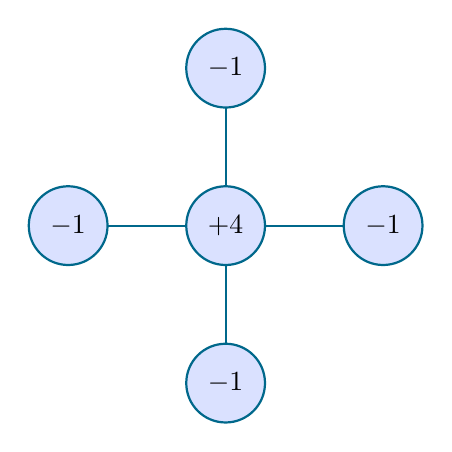
\begin{tikzpicture}[
  every node/.style={
    shape=circle,
    thick,
    fill=cadet,
    draw=darkblue,
    minimum size=1cm,
  }]
  \draw[thick, darkblue] (-2,0) -- (2,0);
  \draw[thick, darkblue] (0,-2) -- (0,2);
  \node at (-2,0) {$-1$};
  \node at (2,0) {$-1$};
  \node at (0,-2) {$-1$};
  \node at (0,2) {$-1$};
  \node at (0,0) {$+4$};
\end{tikzpicture}

    }
  \end{center}

Discretization and implementation of a solver.
\end{frame}

\begin{frame}
  \frametitle{Poisson problem: Diagonalization methods}
  \begin{enumerate}
  \item Compute $\tilde{\bm G}$ using matrix-matrix products
    \begin{equation*}
      \tilde{\bm G} = \bm Q^\intercal \bm G \bm Q.
    \end{equation*}
  \item Solve for $\tilde{\bm U}$.
    \begin{align*}
      \bm \Lambda \tilde{\bm U} + \tilde{\bm U} \bm \Lambda &= \tilde{\bm G} \\
      \lambda_i \tilde{u}_{ij} + \tilde{u}_{ij} \lambda_j &= \tilde{g}_{ij} \\
      \tilde{u}_{ij} &= \frac{\tilde{g}_{ij}}{\lambda_i + \lambda_j}
    \end{align*}
  \item Compute $\bm U$ using matrix-matrix products
    \begin{equation*}
      \bm U = \bm Q \tilde{\bm U} \bm Q^\intercal
    \end{equation*}
  \end{enumerate}

Parallelization of a Poisson solver.
\end{frame}

\begin{frame}
  \frametitle{Direct and iterative solvers}
  \begin{center}
    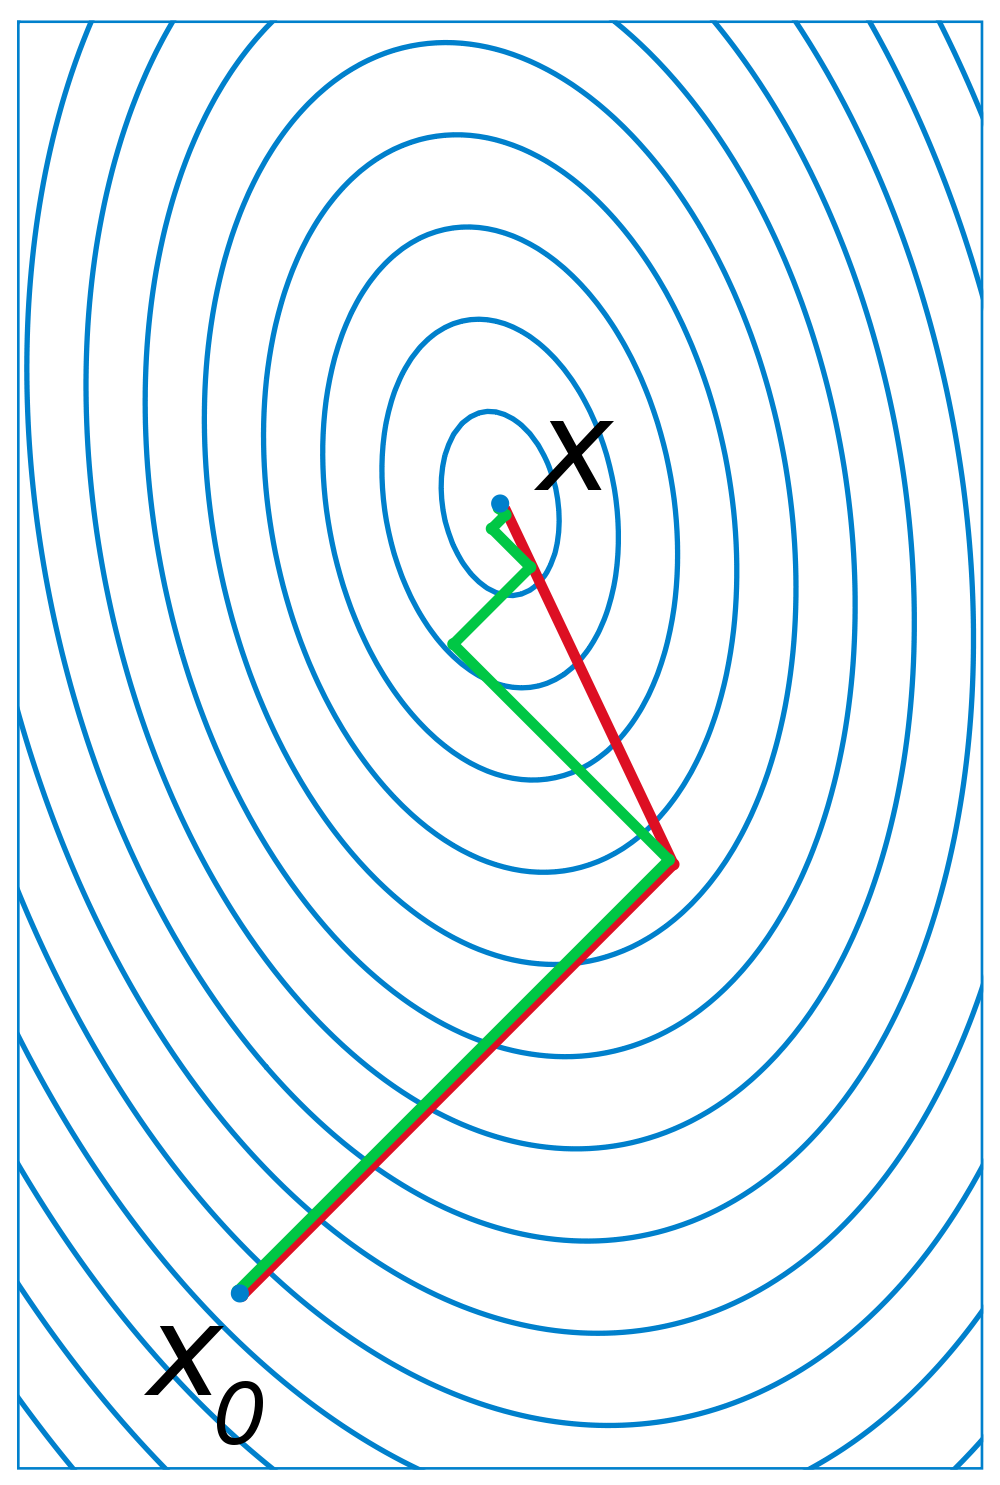
\includegraphics[width=4cm]{\figs/tma4280/cg}
  \end{center}

Overview and performance analysis of direct solvers, descent methods, and Krylov solvers.
\end{frame}

\begin{frame}
  \frametitle{Mesh distribution and domain decomposition}

  \begin{center}
    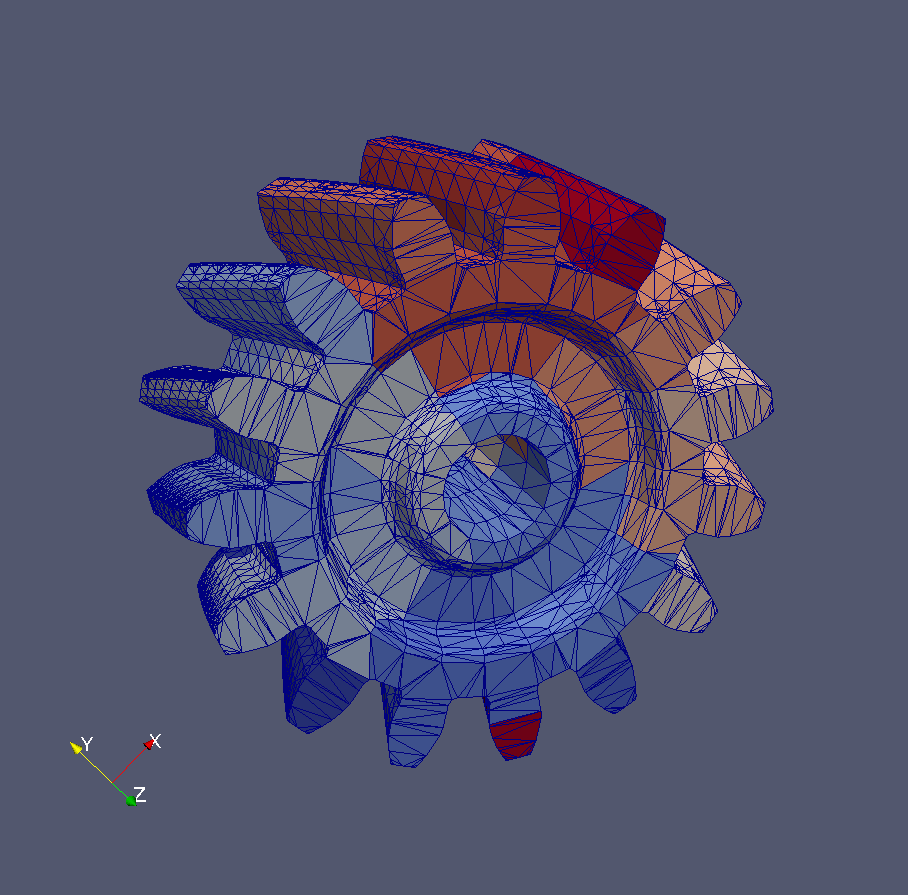
\includegraphics[width=4cm]{\figs/dolfin/gear}
  \end{center}

Review of partitioning techniques for computational meshes \dots
\end{frame}

\begin{frame}
  \frametitle{Parallell I/O with MPI-IO}
  \begin{center}
    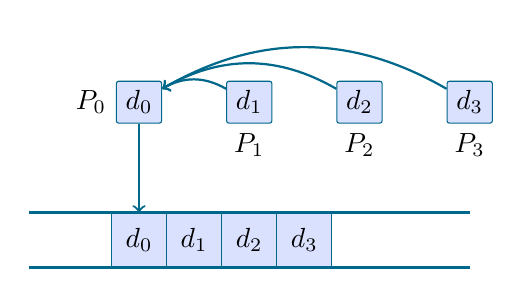
\begin{tikzpicture}[
      scale=0.7,
      data/.style={
        rectangle,
        draw=darkblue,
        fill=cadet,
        rounded corners=0.8,
      }
      ]
      \node[data] (d0) at (0,0) {$d_0$};
      \node[data] (d1) at (2,0) {$d_1$};
      \node[data] (d2) at (4,0) {$d_2$};
      \node[data] (d3) at (6,0) {$d_3$};
      \node[left=0.0 of d0.west] {$P_0$};
      \node[below=0.0 of d1.south] {$P_1$};
      \node[below=0.0 of d2.south] {$P_2$};
      \node[below=0.0 of d3.south] {$P_3$};
      \draw[->, darkblue, thick] (d1) edge[bend right] node [above] {} (d0);
      \draw[->, darkblue, thick] (d2) edge[bend right] node [above] {} (d0);
      \draw[->, darkblue, thick] (d3) edge[bend right] node [above] {} (d0);
      \foreach \i in {0,...,3} {
        \draw[darkblue, fill=cadet] (-0.5+\i, -3) rectangle (0.5+\i, -2);
        \node at (\i, -2.5) {$d_\i$};
      }
      \draw[darkblue, thick] (-2, -3) -- (6, -3);
      \draw[darkblue, thick] (-2, -2) -- (6, -2);
      \draw[darkblue, thick, ->] (d0.south) -- (0,-2);
    \end{tikzpicture}
  \end{center}

\dots and implementation of I/O with MPI.
\end{frame}


\begin{frame}
  \frametitle{Practicalities: Programming, UNIX, Virtual Machine}

\begin{figure}
\centering
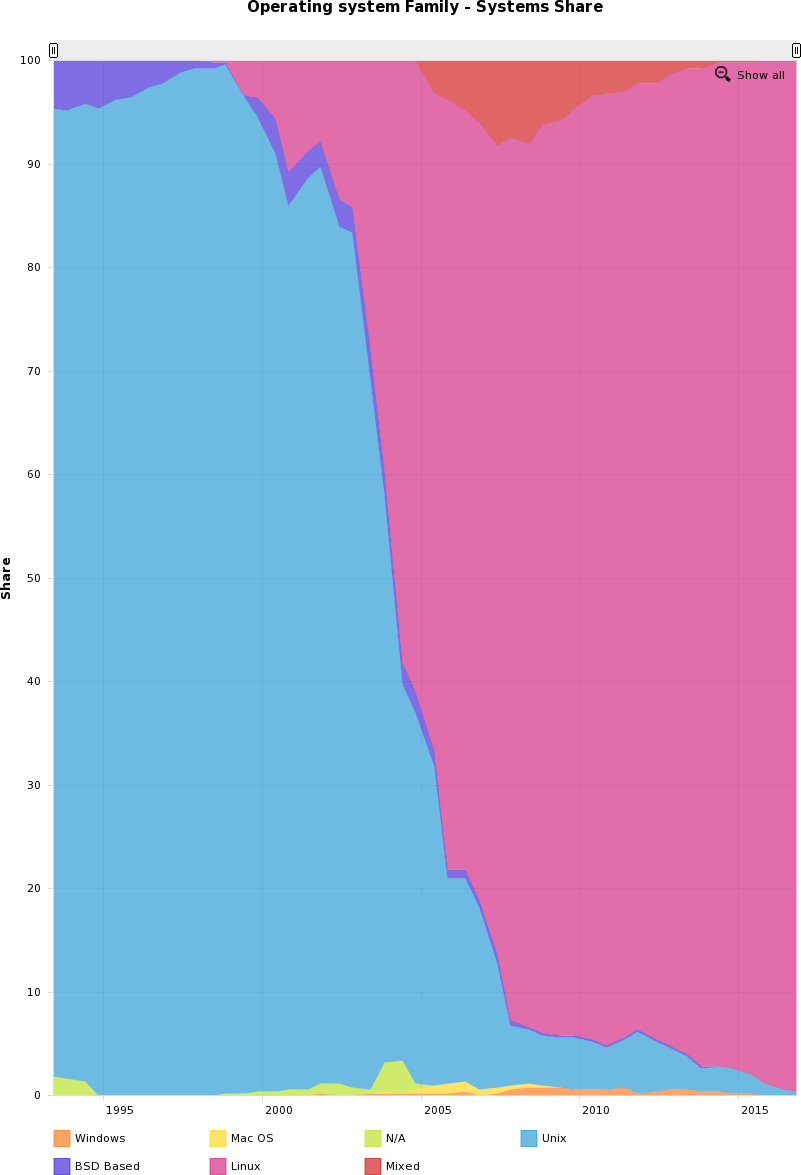
\includegraphics[width=0.4\linewidth]{top500/OS/OS_System}
\caption{Top500: Operating System}
\end{figure}

\end{frame}

\begin{frame}
  \frametitle{Practicalities: Programming, UNIX, Virtual Machine}

Introduction Survey: \url{ https://goo.gl/forms/Sh7nIVRbBo56lgnH3}

\medskip

\begin{itemize}
\item Most supercomputers run GNU/Linux or a flavour of UNIX
\item Software written in C/C++ and FORTRAN mainly
\item Use of Github for projects
\end{itemize}

\medskip

\begin{itemize}
\item Introduction to UNIX on Wednesday January 17. 2018
\item Installation of UNIX environment: virtual machine using Vagrant
\item IRC Channel, \#\#tma4280 on Freenode
\end{itemize}

\end{frame}

\begin{frame}
  \frametitle{Practicalities: Access to IDUN/Lille}

Form for access to supercomputing facilities:
\begin{itemize}
\item Faculty and institute are the ones you belong to, not (necessarily) IME and IMF.
\item Your "local user name" is your NTNU username.
\item Your personal ID is probably <username>@ntnu.no.
\item Leave project number and manager fields blank.
\end{itemize}

Return to me or my mailbox at Sentralbygg II Floor 7 by January 26. 2018.

\end{frame}

\begin{frame}
  \frametitle{Introductory short courses}

Why?
\begin{itemize}
\item Different programme/background with more or less experience with computers.
\item While not a CS course, it is programming intensive.
\item The time required by Projects will depend on your computer fluency. 
\end{itemize}

\medskip
Conclusion: better start getting used to Linux/UNIX as soon as possible!

\medskip
Week 3-4 will not contain any compulsory tasks, but tutorials and training to get everyone onboard!

\end{frame}


% \begin{frame}
%   \frametitle{Heterogeneous computing with CUDA}
%   \begin{center}
%     \texttt{int row = blockIdx.x*blockDim.x+threadIdx.x;}
%   \end{center}
%   \begin{center}
%     
\includegraphics[width=4cm]{cuda}
%   \end{center}
% \end{frame}

\end{document}

